\section{Evaluation}
\label{sec:evaluation}
Our system needs be suitable for economical use. This can be expressed as two requirements: On the one hand, the found joint NER and EL process should find as many correct references as possible to organizations. While Ehmüller~\cite{ehmueller} evaluates this in terms of the standard measures precision, recall and $F_1$ score, we focus on how significant the features are without considering a certain classifier model. On the other hand, our system has to be capable of processing large amounts of data in reasonable time. As our project aims on solving this by means of cluster computing, we evaluate how well the described preprocessing scales out.



\subsection{Significance of the features}
Given a link candidate $lc=(a, c)$ consisting of an alias $a$ and its context $c$ and an entity $en$, the classifier decides whether $lc$ references $en$ or not. Note that, while the link candidate's entity score $es_{en}(a)$ and the context score $cs_{en}(c)$ depend on $en$, $ls(a)$ only depends on the alias itself. Therefore these features must allow a distinction between valid and invalid links regarding the given entity. In the following, I evaluate the distribution of the features based on a sample of 100,000 composite features and how expressive they are for this distinction.

\begin{figure}[ht]
	\begin{tabular}{cc}
	\subfloat[Composite distribution of the entity score and the context score]{
		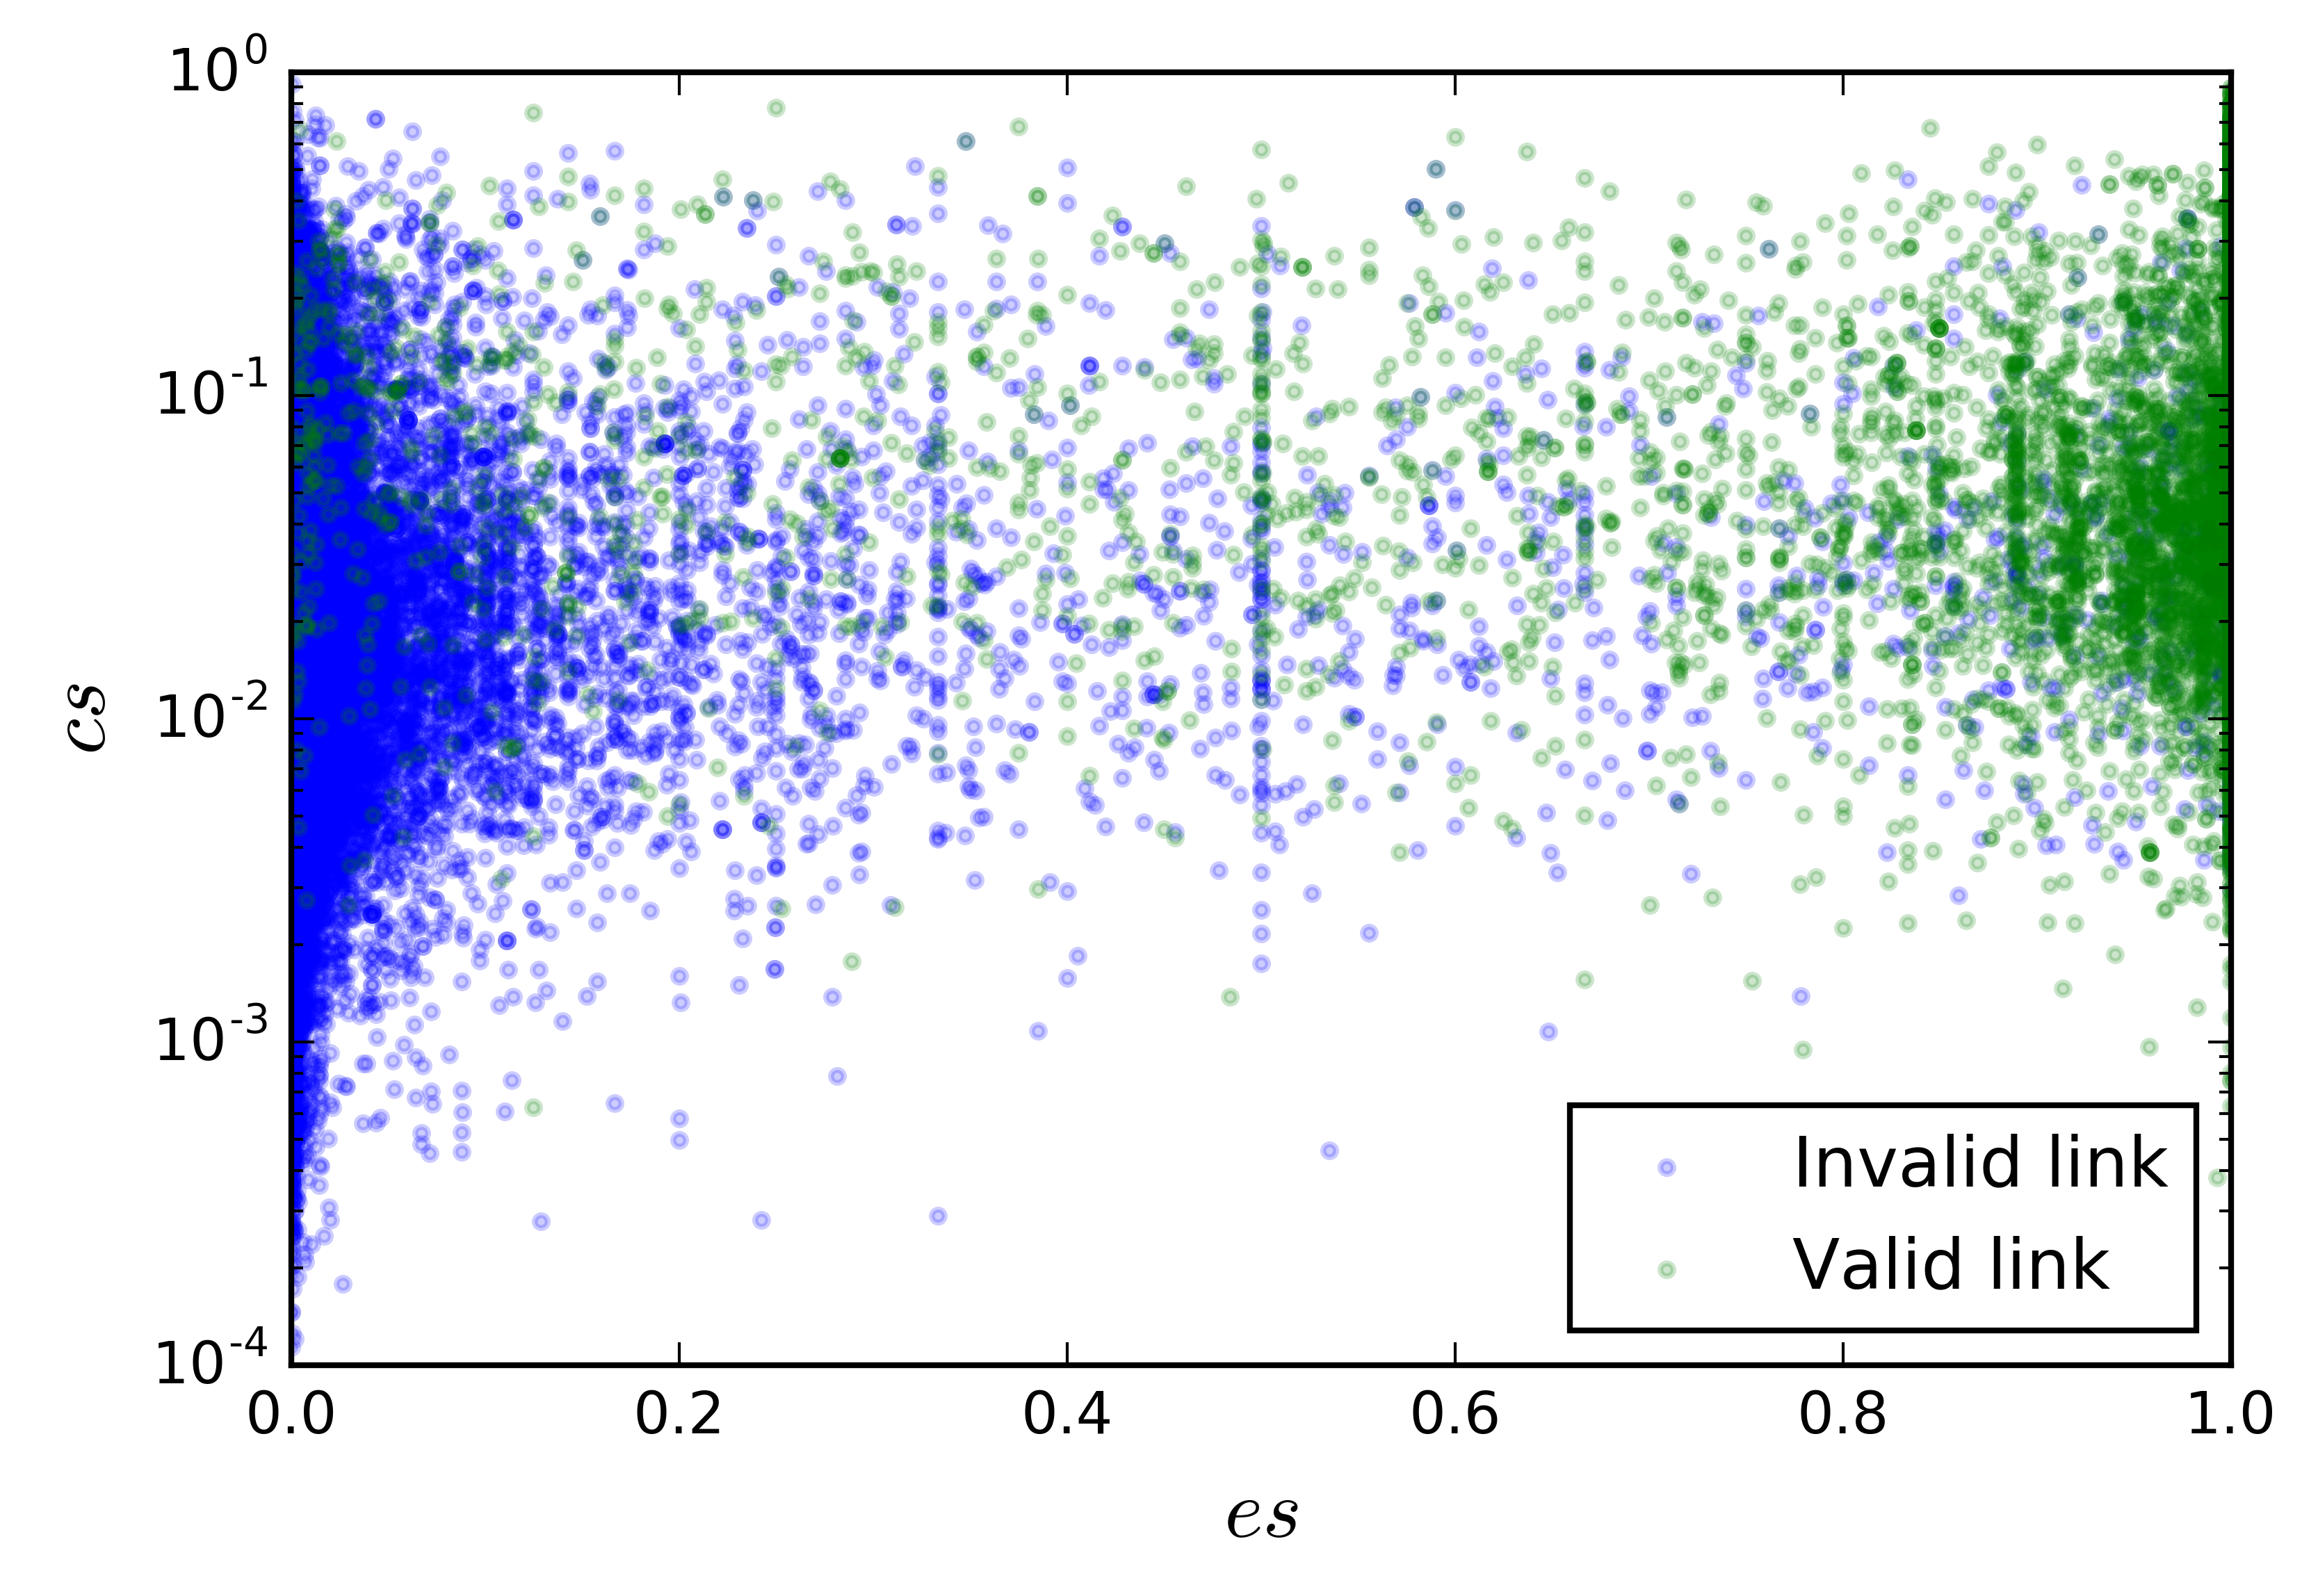
\includegraphics[width = 0.45\textwidth]{Graphics/feature_evaluation/composite_features.png}
		\label{fig:composite_features}
	} &
	\subfloat[Distribtion of the link scores]{
		\includegraphics[width = 0.45\textwidth]{Graphics/feature_evaluation/link_scores.pdf}
		\label{fig:link_scores}
	}\\
	\subfloat[Distribtion of the entity scores]{
		\includegraphics[width = 0.45\textwidth]{Graphics/feature_evaluation/entity_scores.pdf}
		\label{fig:entity_scores}
	} &
	\subfloat[Distribtion of the context scores]{
		\includegraphics[width = 0.45\textwidth]{Graphics/feature_evaluation/context_scores.pdf}
		\label{fig:context_scores}
	}
	\end{tabular}
	\caption{The three used features have significantly different distributions for valid and invalid links.}
	\label{fig:distributions}
\end{figure}

Figure~\ref{fig:composite_features} gives an overview about the composite distribution of the entity score and context score. Note that the context score is scaled logarithmically. The diagram reveals three properties:

\begin{enumerate}
\item There are two clearly identifiable \textbf{clusters}: One for valid links and a high entity score and one for invalid links and a low entity score. 

\item The entity score is more expressive than the context score, as the clusters can only be separated by means of the entity score.

\item There is a \textbf{correlation} between the entity score and the context score: There are far more valid links in the upper right half than in the lower left half of the diagram. This means, that the entity score and context score are "confirming" each other.
\end{enumerate}

Now we consider the features separately to get a more concise understanding of their quality:

\paragraph{Link score}
Figure~\ref{fig:link_scores} shows the distribution of the link scores for the valid and invalid links. Here and in the following, the overlap between the bars is shaded in dark blue. As not more than one entity is valid for each link candidate, our sample contains only 8\% valid links. Thus, for the better visibility, $f$ shows the relative frequency that is 1 both for the valid and invalid links if added up. We can see that a valid link has a link score that is close to 1 in more than 60\% of cases, while invalid links have a link score that is widely distributed. In fact, almost all of the links represented by the last bar have a link score, which is exactly 1. This means, that there are a lot of explicit aliases, which always refer to the same entities. 

\paragraph{Entity score}
Figure~\ref{fig:entity_scores} shows the distribution of the entity scores. he extreme left and extreme right bar represent the clusters observed in Figure~\ref{fig:composite_features}. Thus, the entity score is very expressive for our task. A classifier that decides based on a linear separation between these clusters should yield reasonable results. But since the of valid links is relatively small, this feature is not sufficient.

\paragraph{Context score}
Finally, figure~\ref{fig:context_scores} shows the distribution of the context scores. Note that the frequency is scaled logarithmically. Although there is a large overlap between the valid and the invalid links, the distribution of the valid links is significantly shifted to higher context scores. For a context score of about 0.1, the context score has the least significance. The smaller or higher it becomes from there, the better the classifier can make its decisions.

\paragraph{Second order features}
Also the second order features have a high expressiveness, as shown in Figure~\ref{fig:second_order_features} in the appendix. Similar to the three features described above, they show significantly different distributions for valid and invalid links. Combined with them, the classifier improves the results of our EL even further.


\subsection{Scale out}
\begin{figure}[ht]
	\centering
  \includegraphics[width=\textwidth]{Graphics/ReducedLinkAnalysis2.pdf}
	\caption{Scale out of the link analysis step}
	\label{fig:scale_out}
\end{figure}

In order to make our system scalable for arbitrary input sizes, we use the cluster computing framework Apache Spark\footnotemark{}. As an example for our scale out, Figure~\ref{fig:scale_out} shows the efficiency of our link analysis for a sample of 1,000,000 Wikipedia articles. The efficiency is computed as the average amount of articles that is processed within a second. The scale out was measured for a different number of nodes (i.e., physical computers) and a constant number or CPU cores. A linear scale out would be theoretically perfect. This means that the efficiency increases in the same proportion as the number of nodes. Since there is always communication overhead between the nodes, which increases runtimes, a linear scale or even super-linear scale out is hard to achieve. As we can see, we have an approximately linear scale out for two nodes, but overall, the scale out is sub-linear. The stagnancy for eight nodes might be explained by the relatively small input sample, which leads to an relatively higher communication overhead. The other steps of our preprocessing have similar scale outs.
\footnotetext{\url{https://spark.apache.org/}, last accessed on \formatdate{20}{7}{2017}.}

To contextualize our approach, we compare our approach to a common other implementation for standardized subtasks. This is possible for the computation of the link candidate contexts, which includes the extraction of the bags of words and the subsequent computation of the tf-idf vectors (see Sec.~\ref{sec:context_score}). An alternative implementation is part of the Spark MLlib\footnotemark{}, which was especially designed for cluster computing. 15 runs of both implementations for all links of the German Wikipedia led to an average time of 9.53 minutes for the Spark MLlib and 6.46 minutes for our approach. Therefore, it computes the contexts of link candidates 1.47 times faster than the Spark MLlib.
\footnotetext{\url{https://spark.apache.org/mllib/}, last accessed on \formatdate{20}{7}{2017}.}

~\\

As shown above, the features we use for the extraction of business relations from text have a high quality. They allow a distinction between valid and invalid references to entities. Furthermore, our preprocessing is suitable for cluster computing. It can be distributed over multiple nodes and has an increasing efficiency for a higher amount of computing resources.